\documentclass[11pt]{article}
\usepackage{float}
\usepackage{multirow}
\usepackage[table,xcdraw]{xcolor}
\usepackage{lscape}
\usepackage{longtable}
\usepackage{graphicx}
\usepackage{times}
\usepackage{amsmath}
\usepackage{fdsymbol}
\usepackage{hyperref}
\usepackage[margin=0.6in]{geometry}
\usepackage{multicol}
\usepackage{listings}
\usepackage{xcolor}

\renewenvironment{abstract}
 {\par\noindent\textbf{\abstractname.}\ \ignorespaces}
 {\par\medskip}

\begin{document}

\title{Part C - Privacy Preserving Decision Tree Prediction \\ On Encrypted Data}



\maketitle
\tableofcontents

\newpage

\begin{abstract}
\\ In part C of the project we used secure protocols for prediction and training of tree based models where the data for prediction is encrypted with FHE.
\end{abstract}

\section{Introduction}
Reference to our \href{https://github.com/assiakhateeb/PPML_lab/tree/main/part\%20C}{\textcolor{blue}{Github repo}}.
\\
Part C is an extension to prediction on encrypted data. We implement the prediction by using an adjustment of Algorithm 1.\\
The adjustment is this subroutine which operates over encrypted data :\\

\begin{figure}[H]
\centering
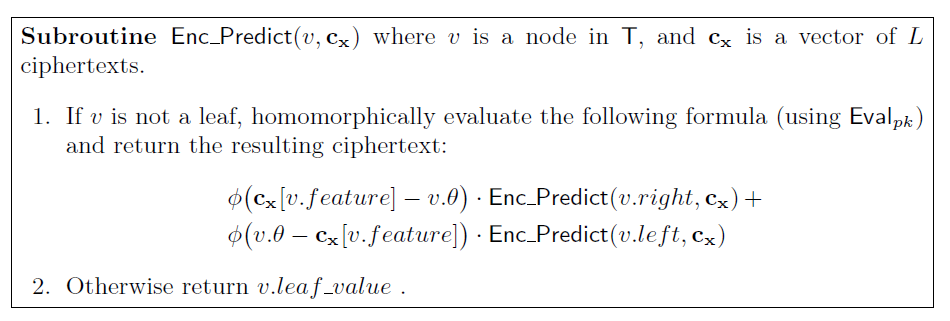
\includegraphics[width=4.7in]{algo1new.PNG}
\caption{}
\label{fig:label}{The subroutine Enc-Predict}
\end{figure}

The protocols that we used are an adaptation of the algorithms in part B but with interactive settings where data is encrypted throughout the computation.\\
See the protocol for prediction over encrypted data in Figures 3 and 4 in Section 4.1 in Akavia's paper.

\section{FHE - Fully Homomorphic Encryption}
Homomorphic Encryption provides the ability to compute on encrypted data.
\par
These resulting computations are left in an encrypted form which, when decrypted, result in an identical output to that produced had the operations been performed on the 'original' data.
\par
This ground-breaking technology has enabled industry to provide capabilities for outsourced computation securely (Homomorphic encryption can be used for privacy-preserving outsourced storage and computation. This allows data to be encrypted and out-sourced to commercial cloud environments for processing, {all while encrypted}).
\par
Homomorphic encryption includes multiple types of encryption schemes that can perform different classes of computations over encrypted data.
\par
The computations are represented as either Boolean or arithmetic circuits. Some common types of homomorphic encryption are partially homomorphic, somewhat homomorphic, leveled fully homomorphic, and fully homomorphic encryption.
\par
\underline{We will use the fully homomorphic encryption scheme}, which allows the evaluation of arbitrary circuits composed of multiple types of gates of unbounded depth, and is the strongest notion of homomorphic encryption. Such a scheme enables the construction of programs for any desirable functionality, which can be run on encrypted inputs to produce an encryption of the result. Since such a program need never decrypt its inputs, it can be run by an untrusted party without revealing its inputs and internal state.
\subsection{Understanding HE}
\begin{itemize}
\item \textbf{“Homomorphic”:} a mapping from plaintext space to ciphertext space that preserves arithmetic operations.
\item \textbf{Mathematical Hardness:} Learning with Errors Assumption; every image (ciphertext) of this mapping looks uniformly random in range (ciphertext space).
\item \textbf{“Security level”:} the hardness of inverting this mapping without the secret key.\\
Example: 128 bits → 2128 operations to break 
\item \textbf{public key (pk):} a key that can be obtained and used by anyone to encrypt messages intended for a particular recipient.\\
\item \textbf{secret key (or “private key”):} a piece of information or a framework that is used to decrypt and encrypt messages. The encrypted messages can be deciphered only by using a second key that is known only to the recipient (the private key).\\
\item \textbf{Plaintext} elements and operations of a polynomial ring. \\
Example: \(3x^5 + x^4 + 2x^3 + ...\)
\item \textbf{Ciphertext} elements and operations of a polynomial ring.\\
Example: \(7862x^5 + 5652x^4 + ...\)
\end{itemize}
\subsection{CKKS Scheme}

CKKS scheme supports efficient rounding operations in encrypted state. The rounding operation controls noise increase in encrypted multiplication, which reduces the number of bootstrapping in a circuit. An important characteristic of CKKS scheme that encrypts approximate values rather than exact values. When computers store real-valued data, they remember approximate values with long significant bits, not real values exactly. CKKS scheme is constructed to deal efficiently with the errors arising from the approximations. The scheme is familiar to machine learning which has inherent noises in its structure.
\subsection{STANDARDIZATION}
There are several reasons why this is the right time to standardize homomorphic encryption.

\begin{itemize}
\item There is a need for easily available secure computation technology as more companies and individuals switch to cloud storage and computing. Homomorphic encryption is already ripe for mainstream use, but the current lack of standardization is making it difficult to start using it.
\item Implementations of leading schemes (CKKS, BFV…) have been adopted to address the needs of privacy-protected computations.

\end{itemize}
Several open-source implementations of homomorphic encryption schemes exist today, we used Microsoft SEAL: A widely used open-source library from Microsoft that supports the BFV and CKKS schemes.

\subsection{TenSeal}
TenSEAL is a library for homomorphic encrypting operations on tensors, built on top of Microsoft SEAL. It provides ease of use through a Python API, while preserving efficiency by implementing most of its operations using C++.


\section{Implementation Details} 
We start by creating a TenSEAL Context for specifying the scheme and the parameters we are going to use.
\subsection{TenSEAL CKKS Context}
\begin{lstlisting}
context = ts.context(ts.SCHEME_TYPE.CKKS, 8192, coeff_mod_bit sizes=[40,21,21,21,21,21,21,40])
\end{lstlisting}
which specifies:
\begin{itemize}
  \item scheme type: ts.SCHEME\textunderscore TYPE.CKKS
  \item poly\textunderscore modulus\textunderscore degree: $8192$.
  \item coeff\textunderscore mod\textunderscore bit\textunderscore sizes: The coefficient modulus sizes, here [60, 40, 40, 60]. This means that the coefficient modulus will contain 8 primes of 40 bits, 6 primes of 21, and last one is 40 bits.
  \item global\textunderscore scale: the scaling factor, here set to $2^{21}$.
  \item generate\textunderscore galois\textunderscore keys: Galois keys are another type of public keys needed to perform encrypted vector rotation operations on batched ciphertexts.
 \end{itemize}
 
\subsubsection{Code}
\begin{lstlisting}
    context = ts.context(ts.SCHEME_TYPE.CKKS, poly_modulus_degree=2 ** 13,
    coeff_mod_bit_sizes=[40, 21, 21, 21, 21, 21, 21, 40]
    )
    context.generate_galois_keys()
    context.global_scale = 2 ** 21

    sk = context.secret_key()
    context.make_context_public()
\end{lstlisting}

\subsection{Trainset Encryption}
\begin{lstlisting}
ts.ckks_tensor(pk,vector)
\end{lstlisting}
The operation encodes vectors of complex or real numbers into plaintext polynomials to be encrypted and computed using the CKKS scheme. It converts a plaintext polynomial to a ciphertext.\\
We encrypt each element of the given trainset using the above command, which specifies:
\begin{itemize}
    \item pk is public key used for encryption.
    \item vector is the element getting encrypted.
\end{itemize}

\subsubsection{Code}
\begin{lstlisting}
    def trainset_enc(X_test,context):
    pk = context.copy()
    encrypted_Xtest = []
    for vec in X_test:
        print(vec)
        encrypted_Xtest.append(ts.ckks_tensor(pk, vec))
    return encrypted_Xtest
\end{lstlisting}

\subsection{Trainset Decryption}
\begin{lstlisting}
decrypt(sk).tolist()
\end{lstlisting}
\begin{itemize}
    \item sk is secret key used for decryption.
\end{itemize}
\subsubsection{Code}
\begin{lstlisting}
    for i in range(len(X_test_encrypted)):
        decrypted_X_test = X_test_encrypted[i].decrypt(sk).tolist()
\end{lstlisting}


\section{Algorithm}
\subsection{Code}
\begin{lstlisting}
    def Tree_Predict_partC(T, x, phi):
    if T is None:
        return
    feature, threshold, leaf, left, right = T.getNode()
    feature = int(abs(feature))
    if isinstance(leaf, np.ndarray):
        return leaf
    else:
        return (x[feature] - threshold).polyval(phi) * Tree_Predict_partC(right, x, phi) + (
            (threshold - x[feature])).polyval(phi) * Tree_Predict_partC(left, x, phi)
\end{lstlisting}
Akavia's algorithm traverses all paths in the tree and computes a weighted combination of all the leaves values, where each leaf value is the 1-hot encoding of the label associated with the leaf. The output is a length L vector assigning a likelihood score to each label, which is in turn interpreted as outputting the label with the highest score.\\
Here we used polyval which is a polynomial evaluation with an encrypted tensor as variable.

\section{Accuracy}
The accuracy is calculated as the percentage of correct classification on test samples. \\
\begin{lstlisting}
algorithm_score = (counter / len(res_vec))*100 
\end{lstlisting}
Counter is equal to the sum of correct classifications and res\_vec is equal to the sum of all classifications.\\ 
\textbf{res\_vec} is the result of the encrypted test set prediction after decrypt and one hot encoding.\\
To know if current classification is correct or not we compare it to Y target value of the relevant sample if they are equal then the prediction of our algorithm is correct . \\

Test samples are decided to be sent to algorithm as 35\% of the samples in the data-set and they are chosen randomly from it.\\
Our algorithm predict over all test samples, after that we calculate accuracy according to the percentage of correct predictions on test samples.\\

\subsection{Code}
\begin{lstlisting}
    def calc_accuracy_partC(res_vec, Y_test):
    counter = 0
    if len(res_vec[0]) == 3:
        for i in range(len(res_vec)):
            if np.logical_and(res_vec[i] == [1, 0, 0], Y_test[i] == 0).all() or np.logical_and(res_vec[i] == [0, 1, 0],Y_test[i] == 1).all() or np.logical_and(res_vec[i] == [0, 0, 1], Y_test[i] == 2).all():
                counter += 1
    if len(res_vec[0]) == 2:
        for i in range(len(res_vec)):
            if np.logical_and(res_vec[i] == [1, 0], Y_test[i] == 0).all() or np.logical_and(res_vec[i] == [0, 1], Y_test[i] == 1).all():
                counter += 1
    return (counter / len(res_vec)) * 100
\end{lstlisting}


\section{Results}

\textbf{Dataset : Iris}\\
\textbf{Max depth : 4}\\
\textbf{Polynom degree : 8 }\\
\textbf{Test size : 30 samples which is 0.2 of the data}\\
\large {Prediction accuracy = 93.33\%}\\
\begin{lstlisting}
X_test =  
    [[-1.66666667e-01 -4.16666667e-01  5.08474576e-02 -2.50000000e-01]
    [-5.00000000e-01  7.50000000e-01 -8.30508475e-01 -1.00000000e+00]
    [-2.22222222e-01 -5.83333333e-01  3.55932203e-01  5.83333333e-01]
    [-7.22222222e-01  1.66666667e-01 -7.96610169e-01 -9.16666667e-01]
    [-6.11111111e-01  1.66666667e-01 -8.30508475e-01 -9.16666667e-01]
    [-2.77777778e-01 -1.66666667e-01  1.86440678e-01  1.66666667e-01]
    [-6.11111111e-01  0.00000000e+00 -9.32203390e-01 -9.16666667e-01]
    .
    .
    .
    [-3.33333333e-01 -7.50000000e-01  1.69491525e-02  2.22044605e-16]
    [-2.77777778e-01 -3.33333333e-01  3.22033898e-01  5.83333333e-01]]
 
Y_test =  [1 0 2 0 0 1 0 ... 1 2]

X_test encrypted = 
    [<tenseal.tensors.ckkstensor.CKKSTensor object at 0x0000024951BEA880>, 
    <tenseal.tensors.ckkstensor.CKKSTensor object at 0x0000024951BEA970>, 
    <tenseal.tensors.ckkstensor.CKKSTensor object at 0x00000249523451C0>, 
    <tenseal.tensors.ckkstensor.CKKSTensor object at 0x00000249523451F0>, 
    <tenseal.tensors.ckkstensor.CKKSTensor object at 0x0000024952345250>, 
    <tenseal.tensors.ckkstensor.CKKSTensor object at 0x0000024952345280>, 
    <tenseal.tensors.ckkstensor.CKKSTensor object at 0x00000249523453D0>,
    .
    .
    .
    <tenseal.tensors.ckkstensor.CKKSTensor object at 0x0000024952345BE0>, 
    <tenseal.tensors.ckkstensor.CKKSTensor object at 0x0000024952345C40>]
    
           ************ Prediction Results *************
           
run time for sample 1 = 15.7883 seconds
predict result for sample 1 =
[0.019447354196179698, 2.864138237961886, 0.6180982373065784]

run time for sample 2 = 15.5750 seconds
predict result for sample 2 =
[1.1053998903954065, 0.6059977397966027, -0.04298346622914129]

run time for sample 3 = 15.4051 seconds
predict result for sample 3 = 
[-0.03223200151966879, 0.4562844833009126, 3.1470747547875613]

run time for sample 4 =15.2020 seconds
predict result for sample 4 =
[1.069321814007992, 0.6582081276819615, 0.002301989696042386]

run time for sample 5 =15.3733 seconds
predict result for sample 5 =
[1.1151917307792774, 0.5585006469020478, -0.013459729121453651]

run time for sample 6 =15.2289 seconds
predict result for sample 6 =
[-0.03276452806617886, 1.7905640163393228, 1.8392962898575334]

run time for sample 7 = 15.1823 seconds
predict result for sample 7 =
[1.2114346531269258, 0.3197190243064703, -0.009674884820227301]
.
.
.
run time for sample 29 = 15.2714 seconds
predict result for sample 29 =
[0.04109668749486619, 2.5464832814579212, 0.895996705268293]

run time for sample 30 = 15.2293 seconds
predict result for sample 30 =
[-0.0240047171361257, 0.4942109706631339, 3.061742831732956]

one hot encoding, prediction result = [
array 1 = ([0., 1., 0.]), 
array 2 = ([1., 0., 0.]), 
array 3 = ([0., 0., 1.]),
array 4 = ([1., 0., 0.]), 
array 5 = ([1., 0., 0.]), 
array 6 = ([0., 0., 1.]), 
array 7 = ([1., 0., 0.]),
.
.
.
array 29 = ([0., 1., 0.]), 
array 30 = ([0., 0., 1.])]
\end{lstlisting}
\newpage
\textbf{Dataset : Cancer}\\
\textbf{Max depth : 4}\\
\textbf{Polynom degree : 8 }\\
\textbf{Test size : 36 samples which is 0.2 of the data}\\
\large {Prediction accuracy = 88.88\%}\\

\begin{lstlisting}
X_test =  
[[-0.58947368 -0.45454545  0.47593583  0.12371134  0.39130435 -0.57241379
  -0.7257384  -0.96226415 -0.27444795 -0.79180887 -0.23577236 -0.27472527
  -0.50499287]
 [-0.77894737 -0.34387352  0.13368984 -0.03092784 -0.43478261  0.32413793
   0.03375527 -0.28301887 -0.10410095 -0.66382253 -0.4796748   0.55311355
  -0.50499287]
 [ 0.07894737  0.24901186  0.06951872  0.12371134 -0.06521739 -0.70344828
  -0.55696203 -0.20754717 -0.53943218  0.38566553 -0.85365854 -0.95604396
  -0.61198288]
 [-0.12631579 -0.68774704 -0.03743316  0.04123711 -0.7826087  -0.72413793
  -0.52742616  0.69811321 -0.23659306 -0.69795222 -0.2195122  -0.42124542
  -0.69044223]
 [-0.11052632 -0.60079051 -0.01604278  0.22680412 -0.69565217 -0.72413793
  -0.40084388  0.32075472 -0.23028391 -0.6552901  -0.3495935  -0.15750916
  -0.70042796]
 [-0.35789474  0.57312253  0.26203209  0.07216495 -0.58695652 -0.72413793
  -0.94514768  0.50943396 -0.75394322 -0.56143345 -0.56097561 -1.
  -0.36947218]
 [ 0.34210526 -0.63636364  0.06951872 -0.12371134 -0.2173913   0.29655172
   0.20253165 -0.66037736 -0.02839117 -0.04095563 -0.00813008  0.17948718
   0.76462197]
.
.
.
.
[ 0.72105263 -0.53359684  0.45454545 -0.03092784  0.08695652  0.25517241
   0.1814346  -0.24528302 -0.01577287 -0.16040956 -0.04065041  0.01098901
   0.42938659]
 [-0.38421053 -0.09486166  0.02673797 -0.13402062 -0.43478261 -0.8137931
  -0.93670886  0.01886792 -0.79810726 -0.27986348 -0.70731707 -0.58974359
  -0.66904422]]

Y_test =  

X_test encrypted = 
[<tenseal.tensors.ckkstensor.CKKSTensor object at 0x0000023917D1B880>,
<tenseal.tensors.ckkstensor.CKKSTensor object at 0x0000023917D1B820>,
<tenseal.tensors.ckkstensor.CKKSTensor object at 0x0000023917D0A0D0>,
<tenseal.tensors.ckkstensor.CKKSTensor object at 0x000002397EDDBFD0>,
<tenseal.tensors.ckkstensor.CKKSTensor object at 0x0000023917D3A190>,
<tenseal.tensors.ckkstensor.CKKSTensor object at 0x0000023917D3AF70>,
<tenseal.tensors.ckkstensor.CKKSTensor object at 0x0000023917CC63D0>,
.
.
.
<tenseal.tensors.ckkstensor.CKKSTensor object at 0x0000023917D55BB0>,
<tenseal.tensors.ckkstensor.CKKSTensor object at 0x0000023917D55C10>]


           ************ Prediction Results *************
           
run time for sample 1 = 15.7645 seconds
predict result for sample 1 =
[0.31465705041981856, 1.4683726550171892, 0.34614773070371824]

run time for sample 2 = 15.4364 seconds
predict result for sample 2 =
[0.5331141271745162, 2.06354218818059, 0.00022079015987372863]

run time for sample 3 = 14.7958 seconds
predict result for sample 3 =
[0.526916049576809, 1.242715732828378, 1.0157657833612563]

run time for sample 4 = 15.0301 seconds
predict result for sample 4 =
[0.10977959931042937, 1.8602146637132575, 0.3252765061893235]
.
.
.
one hot encoding, prediction result = [
array 1 = ([0., 1., 0.]),
array 2 = ([0., 1., 0.]),
array 3 = ([0., 1., 0.]),
array 4 = ([0., 1., 0.]),
array 5 = ([0., 1., 0.]),
.
.
.
]

\end{lstlisting}



\subsection{Conclusions}
We got high accuracy for prediction with
datasets that is encrypted with fully homomorphic encryption, in comparison to standard algorithms on cleartext data.
\par
Prediction is slower (minutes to hours). But,
the protocols we used support real-life enterprise use-cases.

\section{Platforms}
\begin{itemize}
\item pycharm, python 3.9
\item overleaf.com
\end{itemize}

\end{document}